
\subsection*{1.}

\(p(A) = \dfrac{3}{4} = 0{,}75\).

\subsection*{2.}

\begin{center}
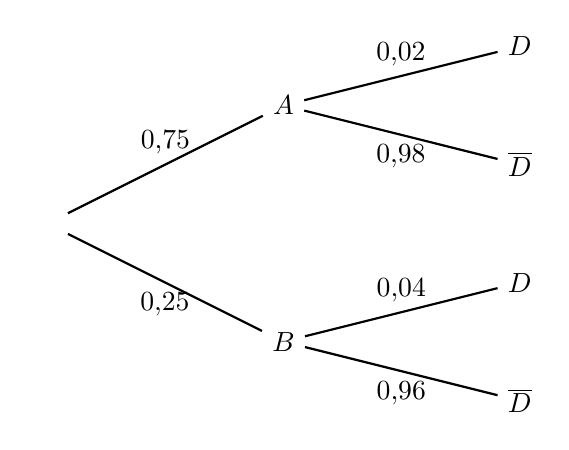
\begin{tikzpicture}[thick, scale=1.5] %{,}
\node (P_-1_0) at (-2,-1.5) {$\phantom{A}$};
\node (P_0_0) at (0,-0.5) {$A$};
\draw (P_-1_0) -- (P_0_0) node[midway, above] {$0{,}75$};
\node (P_1_0) at (2,-0) {$D$};
\draw (P_0_0) -- (P_1_0) node[midway, above] {$0{,}02$};
\node (P_1_1) at (2,-1) {$\overline{D}$};
\draw (P_0_0) -- (P_1_1) node[midway, below] {$0{,}98$};
\node (P_0_2) at (0,-2.5) {$B$};
\draw (P_-1_0) -- (P_0_2) node[midway, below] {$0{,}25$};
\node (P_1_2) at (2,-2) {$D$};
\draw (P_0_2) -- (P_1_2) node[midway, above] {$0{,}04$};
\node (P_1_3) at (2,-3) {$\overline{D}$};
\draw (P_0_2) -- (P_1_3) node[midway, below] {$0{,}96$};
\end{tikzpicture}
\end{center}

\subsection*{3.}

Il faut calculer :
\[
p(D \cap A) = p(A \cap D) = p(A) \times p_A(D) = 0{,}75 \times 0{,}02 = 0{,}015.
\]

\subsection*{4.}

On a aussi :
\[
p(D \cap B) = p(B \cap D) = p(B) \times p_B(D) = 0{,}25 \times 0{,}04 = 0{,}01.
\]

D'après la loi des probabilités totales :
\[
p(D) = p(D \cap A) + p(D \cap B) = 0{,}015 + 0{,}01 = 0{,}025.
\]

\subsection*{5.}

Il faut calculer :
\[
p_D(A) = \dfrac{p(D \cap A)}{p(D)} = \dfrac{0{,}015}{0{,}025} = \dfrac{15}{25} = 0{,}6.
\]

